%! Author = Stepan Oskin
%! Date = 2019-07-31

% Preamble
\documentclass[11pt]{article}
\usepackage{subcaption}
\usepackage{graphicx}

% Packages

% Document
\begin{document}

    \title{Teranet database \\
    OSEMN methodology \\
    Step 3: Explore \\
    Results of Exploratory Data Analysis}
    \author{Stepan Oskin}

    \maketitle

    \begin{abstract}
    Discussion of the results of Exploratory Data Analysis (EDA) of Teranet data.
    \end{abstract}

    \section{Drastic change in the number of transactions recorded per year between 1984 and 1985} \label{sec:num_records_change}

    As a part of the Exploratory Data Analysis of Teranet records, alpha shapes have been produced from yearly subsets of Teranet data.
    In addition, the count of real estate transactions recorded per year in Teranet database has been added for each municipality.
    Upon examination, the resultant shapes and record counts show a dramatic increase in the number of recorded real estate transactions for every GTHA municipality between years 1984 and 1985.
    For example, there is a total of only 68 transactions recorded in the City of Toronto in 1984, while there is 4'222 transactions recorded in Toronto in 1985, which constitutes a 6'208\% increase year-on-year in the count of records.
    Similar change can be observed across every GTHA municipality, with consistently low number of transactions recorded every year prior to 1985, and consistently high number of transactions recorded every year afterwards.
    This "boundary" can be seen on figures~\ref{fig:teranet_as_1984} and~\ref{fig:teranet_as_1985}.

    \begin{figure}[hbt!]
        \centering
        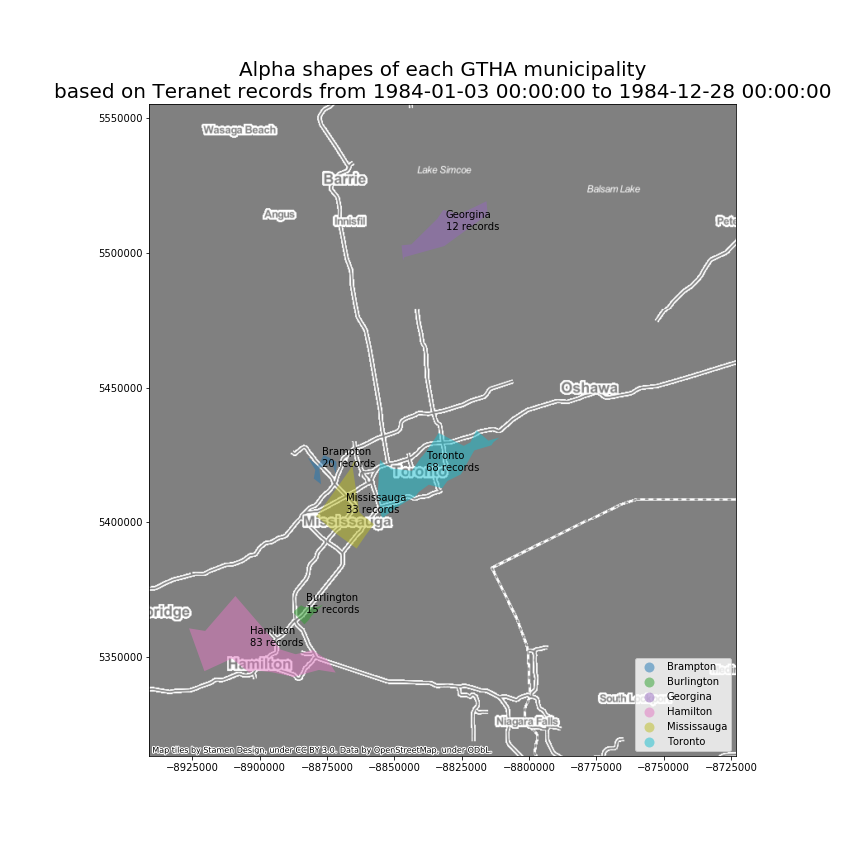
\includegraphics[width=1\linewidth,trim=0.5 0.5 0.5 0.5,clip]{img/as_1984-01-03_1984-12-28.png}
        \caption{Alpha shapes and count of transactions recorded by Teranet in 1984.
        The counts of records is representative of each year prior to 1985.}
        \label{fig:teranet_as_1984}
    \end{figure}


    \begin{figure}[hbt!]
        \centering
        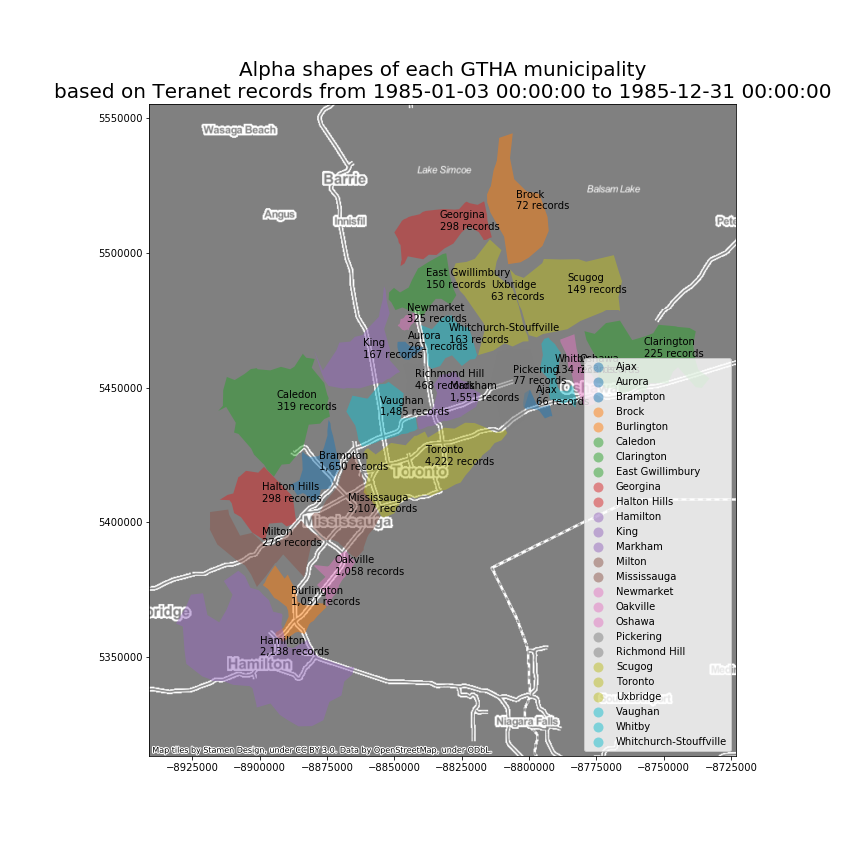
\includegraphics[width=1\linewidth,trim=0.5 0.5 0.5 0.5,clip]{img/as_1985-01-03_1985-12-31.png}
        \caption{Alpha shapes and count of transactions recorded by Teranet in 1985.
        The count of records is representative of each year after 1985.
        The drastic change in counts of recorded transactions seems to coincide with the introduction of POLARIS system by the Government of Ontario in 1985.}
        \label{fig:teranet_as_1985}
    \end{figure}
    The change in the count of records seems to coincide in time with the introduction of the Province of Ontario Land Registration Information System (POLARIS) by the Government of Ontario, which occurred in 1985.

\end{document}